\section{Odwzorowania i ich własności}
\begin{definicja}\label{DefFunkcji}
Niech $A,B$ będą danymi zbiorami. Przyporządkowanie każdemu elementowi $x$ ze zbioru $A$ dokładnie jednego elementu $y$ ze zbioru $B$ nazywamy odwzorowaniem, bądź funkcją, ze zbioru A w zbiór B. Zależność tą oznaczamy w następujący sposób: $$f(x)=y$$ 
\end{definicja}
\begin{definicja}
Elementy ze zbioru $A$, z definicji \ref{DefFunkcji} nazywamy argumentami \index{Argumenty funkcji} funkcji $f$.
\end{definicja}

\begin{definicja}
Zbiór argumentów funkcji $f$ nazywamy dziedziną \index{Dziedzina funkcji} funkcji $f$.
\end{definicja}


\begin{definicja}
Zbiór $B$, z definicji \ref{DefFunkcji} nazywamy przeciwdziedziną \index{przeciwdziedzina funkcji} funkcji $f$.
\end{definicja}


Przydatne będzie następujące oznaczenie:
\begin{definicja}
Niech $f$ będzie funkcją określoną jak w definicji \ref{DefFunkcji}. Ponadto, niech $C \subset A$, wtedy:
$$f(C) = \{f(c) \in B : c \in C \} $$
Zbiór ten nazywamy, obrazem zbioru $C$.
\end{definicja}

\begin{definicja}
Niech $f$ będzie funkcją określoną jak w definicji \ref{DefFunkcji}. Wtedy zbiór
$$ Y = f(A) $$
nazywamy zbiorem wartości funkcji.
\end{definicja}

\begin{cor}
Na ogół terminy: zbiór wartości funkcji oraz przeciwdziedzina uznaje się za równoważne.
\end{cor}

\begin{definicja}
Niech $f$ będzie funkcją określoną jak w definicji \ref{DefFunkcji}. Ponadto, niech $D \subset B$, wtedy:
$$f^{-1}(D) = \{a \in A : f(a) \in D \} $$
Zbiór ten nazywamy, przeciwobrazem zbioru $D$.
\end{definicja}

\begin{definicja}
Wykresem odwzorowania $f:X\rightarrow Y$ nazywamy zbiór $\Gamma_{f}=\{(x,y):x\in X \land y=f(x)\}$
\end{definicja}


Teraz zobaczmy kilka przykładów zastosowania powyższych definicji w praktyce. Będziemy używali oznaczeń takich jak w definicji \ref{DefFunkcji}.

\begin{przyklad}
Niech
$$y=f(x)=x^2$$
$$ A = <-1;1> $$
$$ B = <0;1> $$

\begin{figure}[h!]
  \begin{center}
    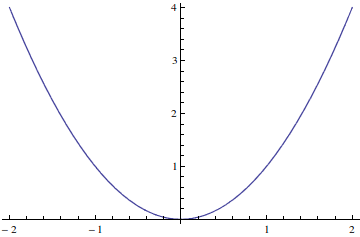
\includegraphics[width=0.48\textwidth]{./podrozdzial01-obrazki/parabola.png}
  \end{center}
  \caption{Wykres funkcji $ y=x^2 $}
\end{figure}
Jak wygląda przeciwobraz zbioru $<\frac{1}{4},1> $?

\begin{figure}[H]
  \begin{center}
    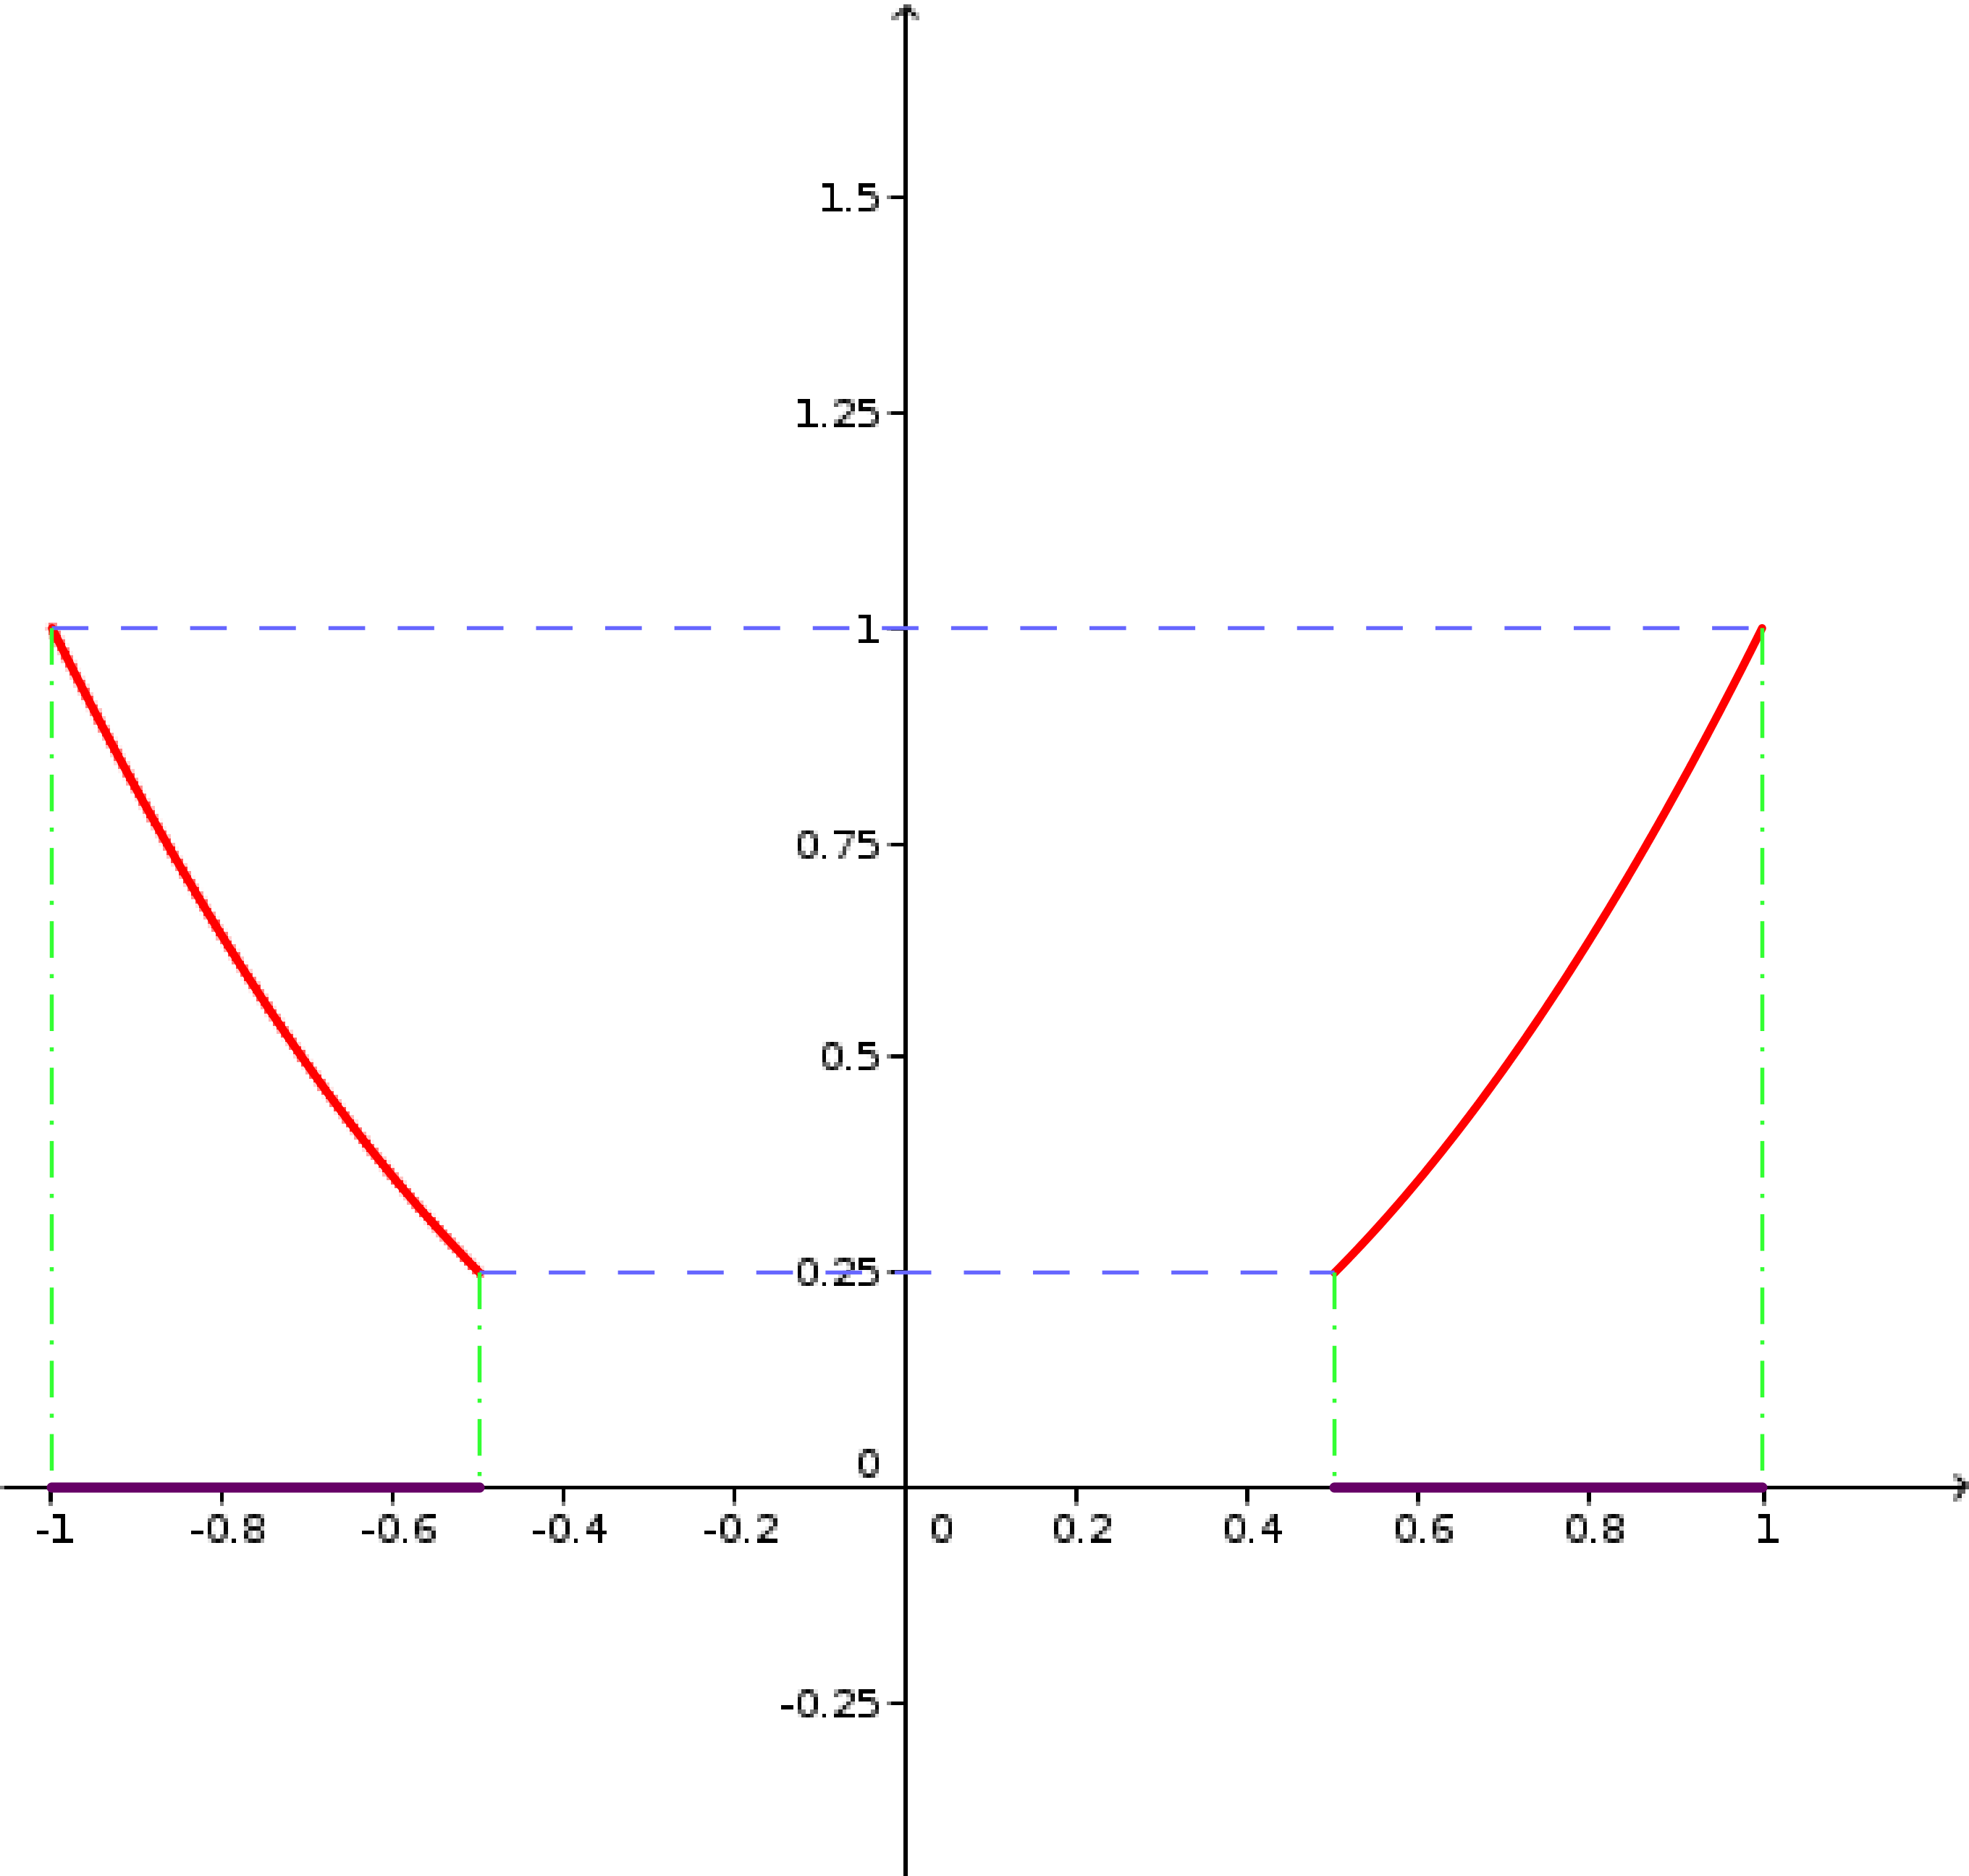
\includegraphics[width=0.48\textwidth]{./podrozdzial01-obrazki/przeciwobraz-parabola.png}
  \end{center}
  \caption{Odczytywanie przeciwobrazu zbioru $<\frac{1}{4},1> $ względem odwzorowania $ y=x^2 $}
\end{figure}
Stąd widać, że $f^{-1}(<\frac{1}{4},1>)= <-1,-\frac{1}{2}> \cup <\frac{1}{2},1> $.
\\Podobnie, łatwo odczytujemy, że $f^{-1}(<0,1>)= <-1,1>$.
\end{przyklad}

Teraz sprwdźmy jak to wygląda dla funkcji liniowych.
\begin{przyklad}
$y=2x+1 $,
\\ Tutaj z kolei mamy $A=\mathbb{R} $, oraz $B = \mathbb{R}$.
\begin{figure}[H]
  \begin{center}
    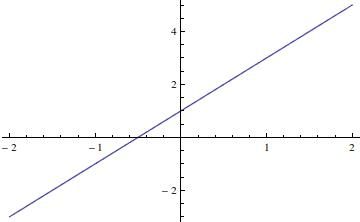
\includegraphics[width=0.48\textwidth]{./podrozdzial01-obrazki/funkcja-liniowa.jpg}
  \end{center}
  \caption{Wykres funkcji $y=2x+1$}
\end{figure}


\end{przyklad}

\begin{przyklad}
$y=\sin(x) $,
\\ Tutaj z kolei mamy $A=\mathbb{R} $, oraz $B = <-1,1>$.
\begin{figure}[H]
  \begin{center}
    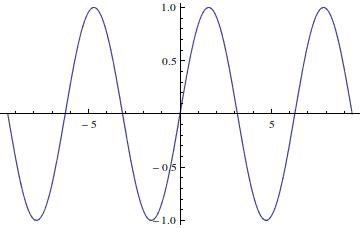
\includegraphics[width=0.48\textwidth]{./podrozdzial01-obrazki/funkcja-sinus.jpg}
  \end{center}
  \caption{Wykres funkcji $y=\sin(x)$}
\end{figure}
\end{przyklad}

\begin{przyklad}
$y=[x] $ - funkcja ta każdej liczbie $x$ przyporządkowuje największą liczbę całkowitą, nie większą od $x$.
\\ Tutaj z kolei mamy $A=\mathbb{R} $, oraz $B = \mathbb{Z}$.
\begin{figure}[H]
  \begin{center}
    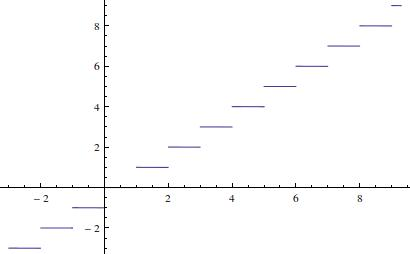
\includegraphics[width=0.48\textwidth]{./podrozdzial01-obrazki/funkcja-cecha.jpg} % #TODO: dopracować wykres - końce przedziałów!
  \end{center}
  \caption{Wykres funkcji $y=[x]$}
\end{figure}

\end{przyklad}





\begin{definicja}
Złożeniem odwzorowań $f:X\rightarrow Y$ i $g:Y\rightarrow Z$ nazywamy odwzorowanie $h=g\circ f:X\rightarrow Z$ takie, że dla każdego $x \in X$, zachodzi $ (g\circ f)(x)=g(f(x))$.
\end{definicja}
\begin{definicja}
Niech $f:X\rightarrow Y \land A\subset X$. Odwzorowanie $g:A\rightarrow Y$ nazywamy zawężeniem (restrykcją) funkcji $f$ do zbioru $A$, jeśli dla każdego $x \in A$ zachodzi równość  $ g(x) = f(x)$.
\end{definicja}

\begin{definicja}%inj
Niech $f:X\rightarrow Y$. Odwzorowanie $f$ nazywamy injekcją, jeżeli

$$\forall x_{1},x_{2} \in X : x_{1} \neq x_{2} \Rightarrow f(x_{1}) \neq f(x_{2}) .$$
\end{definicja}

\begin{ozn}
Zamiast pojęcia injekcja, często można spotkać się z nazwami takim jak: odwzorowanie jednokrotne lub różnowartościowe. Wszystkie te pojęcia są równoważne.
\end{ozn}

\begin{definicja}%surj
Niech $f:X\rightarrow Y$. Odwzorowanie $f$ nazywamy surjekcją (lub "odwzorowaniem na"), jeżeli $f(X)=Y$.
\end{definicja}


\begin{definicja}%bij
Jeśli odwzorwanie $f$ jest surjekcją oraz injekcją, to $f$ nazywamy bijekcją albo odwzorowaniem wzajemnie jednoznacznym.
\end{definicja}

\begin{przyklad}
Niech $A = A_1 \times A_2 \times \dots \times A_n $.
Zdefiniujmy następujące odwzorowania:
$$P_j : A \rightarrow A_j : P_j(a_1,a_2, \dots ,a_n)=a_j \text{ , dla  } j = 1, \dots ,n .$$
Funkcję taką nazywamy projekcją zbioru $A$ na zbiór $A_j$.

$P_j$ jest surjekcją na $A_j$, jeśli $A_j \neq \emptyset$. 
 
\end{przyklad}

\begin{przyklad}
Weźmy $f(x) = 2^x$, $x \in \mathbb{R}$.
\begin{figure}[H]
  \begin{center}
    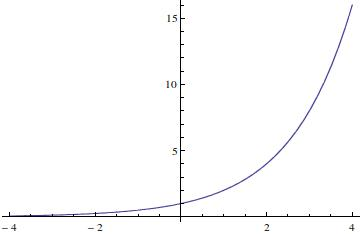
\includegraphics[width=0.48\textwidth]{./podrozdzial01-obrazki/1.jpeg}
  \end{center}
  \caption{Wykres funkcji $y=2^x$}
\end{figure}
To odwzorowanie jest injekcją.

\end{przyklad}

\begin{przyklad}
Weźmy $f(x) = \tan(x)$, $x \in (-\frac{\pi}{2},\frac{\pi}{2})$.
\begin{figure}[H]% #TODO: Rysunek!!
  \begin{center}
    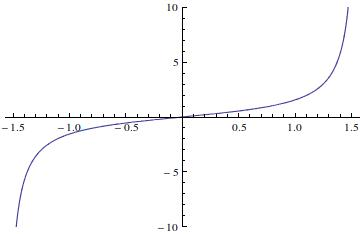
\includegraphics[width=0.48\textwidth]{./podrozdzial01-obrazki/2.jpeg}
  \end{center}
  \caption{Wykres funkcji $y=\tan(x)$}
\end{figure}
Mamy tutaj $f((-\frac{\pi}{2},\frac{\pi}{2})) = \mathbb{R} $, zatem odwzorowanie to jest surjekcją.
Łatwo zauważyć, że przy tak dobranej dziedzinie, odwzorowanie to jest również injekcją. 
Stąd $f$ jest surjekcją.

\end{przyklad}

\begin{ozn}
Niech $f: X \rightarrow Y$. Przez $I_X$ oznaczamy odwzorowanie identycznościowe w zbiorze $X$, tzn., że $I_X: X \rightarrow X$ oraz dla każdego $x\in X$ zachodzi $ : I_X(x)=x $. Analogicznie definiujemy identyczność w $Y$
\end{ozn}

\begin{definicja}
Jeśli odwzorowania $f: X \rightarrow Y $,  $g: Y \rightarrow X $, spełniają warunki:
\begin{itemize}
\item $ g \circ f = I_X  $, tzn. $g(f(x))=x $, dla każdego $x \in X$, \label{zlozenieWarunek1}
\item $ f \circ g = I_Y  $, tzn. $f(g(y))=y $, dla każdego $y \in Y$,
\end{itemize}
to odwzorowanie $g$ nazywamy odwrotnym do $f$ i na odwrót.
\end{definicja}

Można to zobrazować za pomocą następującego rysunku:


\begin{figure}[H]% #TODO: Rysunek!!
  \begin{center}
    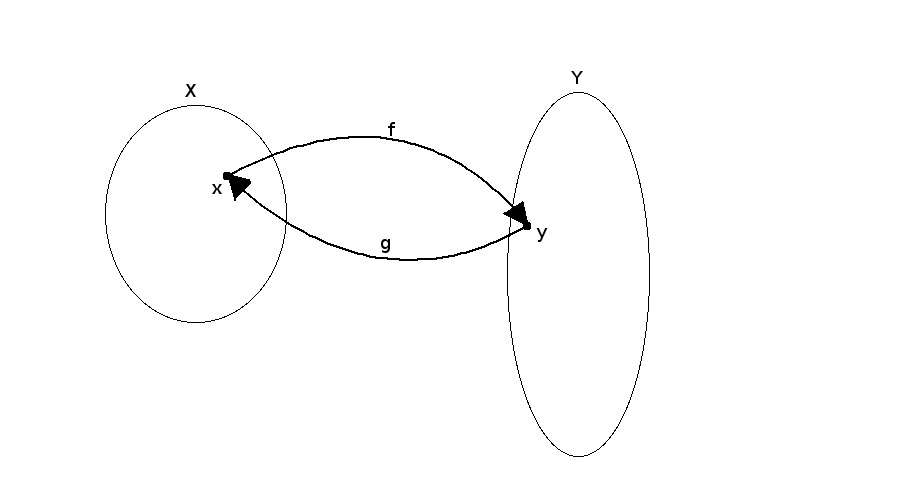
\includegraphics[width=0.88\textwidth]{./podrozdzial01-obrazki/3.png}
  \end{center}
  \caption{Zależność pomiędzy funkcją, a jej odwrotnością.}
\end{figure}

\begin{ozn}
Odwzorowanie odwrotne do $f$ oznacza się jako $f^{-1}$.
\end{ozn}
Oznaczenie to mocno kojarzy się z przeciwobrazem zbioru poprzez funkcję. Te pojęcia są ze sobą związane. Żeby zapoznać się z pojęciem odwzorowanie odwrotnego oraz dostrzec pewne różnice między nimi, przeanalizujmy przykłady.

\begin{przyklad}
$f: X \rightarrow X$, gdzie $f = I_X$,
\\ Tutaj $f^{-1}=I_X$.
\end{przyklad}

\begin{przyklad}
$f: [-1;1] \rightarrow [0;1]$, gdzie $f = x^2$,
\\ Tutaj z kolei $f^{-1}$ nie istnieje!. Wynika to z faktu, że $f$ nie jest odwzorowaniem różnowartościowym.
\begin{figure}[H]% #TODO: Rysunek!!
  \begin{center}
    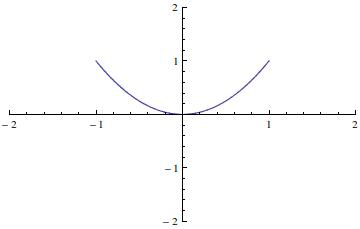
\includegraphics[width=0.48\textwidth]{./podrozdzial01-obrazki/4.jpeg}
  \end{center}
  \caption{Wykres funkcji $y=\sin(x)$}
\end{figure}
Rzeczywiście, jedynym kandydatem na funkcję odwrotną wydaje się funkcja $g(y) = \sqrt{y}$, bo mamy:
$$f \circ g (y) = y ,$$
jednak z drugiej strony, mamy:
$$ g \circ f (x) \neq x  \text{  dla  } x<0 ,$$
zatem pierwszy warunek z definicji \ref{zlozenieWarunek1}, nie jest spełniony.

\end{przyklad}



%%%%%%%% Do skopiowania:

%